The fact that matter responds to gravitational waves as described
in section~\ref{sec:effects_of_waves} offers the possibility of making
a direct detection of such waves.  Although several methods of
detection have been proposed, we focus here on that used by LIGO and,
with some differences, Virgo and GEO.  Again, this presentation will
be of necessity brief.  We refer readers to the textbook by
Saulson~\cite{Saulson:1994} for a much more comprehensive
treatment.

Throughout this and the following chapters we will refer to 
the entire apparatus as an \emph{Interferometric Observatory}
(IFO), \emph{detector} and \emph{instrument} interchangeably.

\section{A Toy Model}

We motivate our discussion of the LIGO interferometers with a toy
model.  We wish to detect gravitational waves, and one method is
suggested by the analysis of the preceding chapter; we look for the
strain, $\Delta L/L$, by measuring change in length of some system.
Simply measuring a length with a ruler will not work, as any ruler
will itself be stretched and compressed by the wave.  However, we can
also measure distance by sending a projectile, say a marble, with
known velocity through the length and measuring the travel time.  To
avoid complex issues of synchronizing clocks at different points in
general relativity we add a (hypothetical perfectly elastic) rubber
wall at the far end, and measure how long it takes to return.  If the
velocity of the marble is much larger than the velocity of the wall
induced by the wave (that is, $v \gg h \omega L$ where $h$ is the
strain and $\omega$ the gravitational wave frequency) then there is a
simple relationship between the round-trip travel time and the
amplitude of the wave.

However, this requires unrealistic precision in measurement, the
uncertainty in the marbles' launch time will swamp the small changes in 
length since, as we will see in the next chapter, $h$ is typically
very small.

Therefore, we instead construct a \emph{null experiment} where we try
to determine if a given quantity is exactly zero.  We arrange two
perpendicular paths, fire marbles down each at the same time and
measure the difference in return times.  As gravitational waves are
rare, we ``lock'' the system by shifting one or both of the walls such
that the marbles always collide exactly (say by measuring their recoil
angle).  Once locked, deviations in the length of either or both arms
will cause the difference in arrive times to become non-zero, which
can be determined by a change in the marbles' recoil angles or lack of
collision entirely.

To obtain robust results we want $\delta L$ to be as large as
possible.  Since gravitational waves are week, this means increasing
$L$.  Practical concerns may limit the ability to do this.  For
example, clearly the entire path from source to walls must be in
vacuum in order for the marbles not to lose energy, and building large
vacuum systems is difficult and expensive.  We therefore use a trick
and add a second set of walls between the source and reflectors, and
arrange the paths so that the marbles bounce back and forth several
times before returning to the source.  This effectively extends $L$ by
the distance between the two surfaces multiplied by the number of
bounces.

Our final extension to this toy model is rather unrealistic, but
imagine that marbles vanish after a collision.  Our ability to detect a
gravitational wave with statistical confidence then reduces to our
ability to count marbles.  We can model this as a Poisson process, where
probability of observing $N$ marbles is 

\begin{equation*}
p(N) = \frac{\bar{N}^N \exp(-\bar{N})} {N!}
\end{equation*}

where $\bar{N}$ is the average expected number of marbles per
observation period.  The error in estimating $N$ from counting goes as
$1/\sqrt{N}$, and it is therefore advantageous to send out as many 
marbles as possible.

\section{Interferometric Gravitational Wave Detectors}

The toy model presented above captures the essential principles behind
LIGO, with the significant difference that light is used instead of
marbles.  A cartoon of the LIGO instruments is shown in
figure~\ref{f:ligo}.  The laser, beam splitter and two outer mirrors
(labeled \texttt{ETMX} and \texttt{ETMY} for ``end test masses'') form
a \emph{Michelson interferometer}, and parallel the original toy model
with two marbles and two reflecting surfaces.


\begin{figure}
  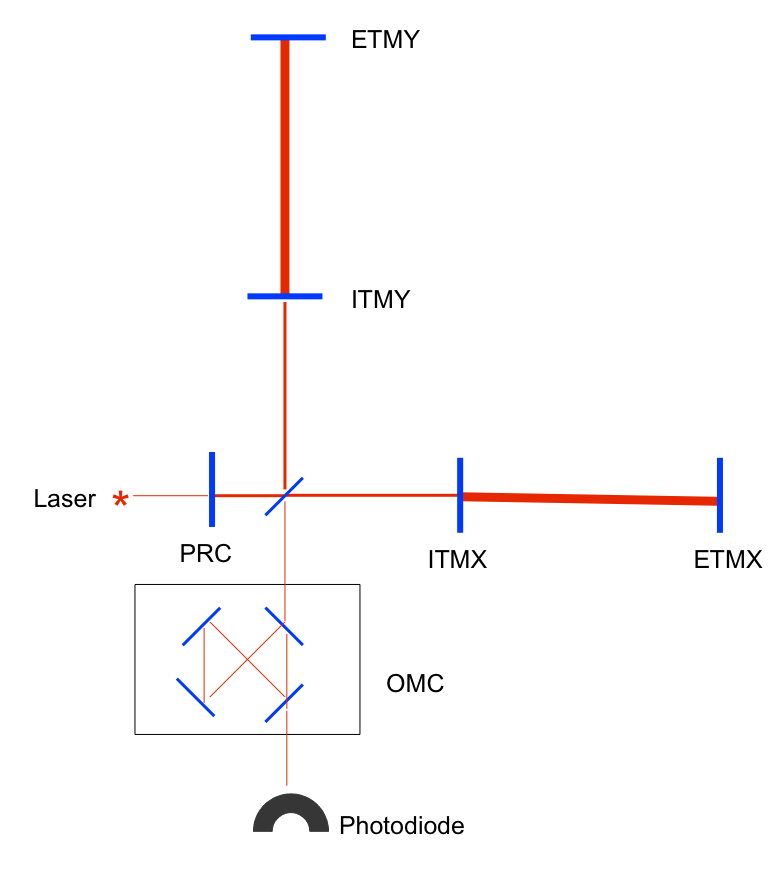
\includegraphics[width=\linewidth]{figures/detectors/LIGO}
  \caption[Block diagram of LIGO]{
  \label{f:ligo}
Block diagram of LIGO, see the text for description.
}
\end{figure}%
The use of light actually simplifies the analysis because light
travels on null geodesics, so

\begin{equation*}
ds^2 = 0 = g_{\mu\nu} dx^\mu dx^\nu
\end{equation*}

We now consider a +-polarized gravitational wave travelling in the $z$
direction, and place the arms on the $x$ and $y$ axes.  We again
assume the frequency of the wave is large compared to the travel time
between the arms, which implies that, over the round trip, $h_+$ may be
taken to be constant and the metric becomes

\begin{equation*}
g_{\mu\nu} = -dt^2 + (1+h_+) dx^2 + (1-h_+) dy^2 + dz^2
\end{equation*}

Then for the $x$ axis, restoring physical units,

\begin{equation*}
c^2 dt^2 = (1+h_+) dx^2
\end{equation*}

and the round-trip travel time is

\begin{equation*}
t_x = \frac{2L}{c} \sqrt{1+h_+} \approx \frac{2L}{c} \left(1+\frac{h_+}{2} \right)
\end{equation*}

where we approximate the square root by its taylor series and ignore
higher-order terms in $h_+$.

Similarly the round-trip light travel time along the $y$ arm is

\begin{equation*}
t_y = \frac{2L}{c} \left(1-\frac{h_+}{2} \right)
\end{equation*}


Considering a single wavefront leaving the beam splitter, the
difference in return time is

\begin{equation*}
\Delta t = t_x - t_y = \frac{2L}{c} h_+
\end{equation*}

In interferometry what matters is not the difference in arrival time
of a wave front, but the difference in phase.  This difference will
cause an interference pattern that will serve as the readout.  If we
use laser light of frequency $f$ and wavelength $\lambda = c/f$ then a
time difference of $\Delta t$ corresponds to a phase difference of 

\begin{equation*}
\Delta \Phi = \frac{2\pi f}{\Delta t} = \frac{4\pi f L}{c} h_+
= \frac{4\pi L}{\lambda} h_+
\end{equation*}

As in the marble example, we can increase the sensitivity of the
instrument by increasing $L$, but practical considerations prevent us
from doing so.  One of these considerations is in fact the same for
marbles and light; the travel path must be in vacuum.  We
therefore employ the same trick and add two additional mirrors,
indicated as \texttt{ITMX} and \texttt{ITMY} (for ``initial test
masses'').  The addition of these mirrors creates a \emph{Fabry-Perot
cavity} in each arm.  By arranging the mirrors to be an integer
number of wavelengths apart a resonance is built up that can trap the
light for extended periods, approximately 200 bounces.  It can be seen
that if the mirrors are not appropriately spaced there will be
destructive interference between the light moving in different
directions.  As the power in the beam must be conserved, this results
in energy leaking out of the cavity, reducing the efficiency.

The addition of the Fabry-Perot cavities would suggest an increase in
phase difference of two orders of magnitude.  However, it is in fact
better than that.  The light is now in flight sufficiently long that,
for gravitational waves from astrophysical sources, $h_+$ will have
changed during the interval and the above analysis is no longer
valid.  A more careful analysis shows that the improvement is 
three orders of magnitude.

In interferometry it is typically most useful to think of light as a
wave.  However, where in the toy example our ability to detect
gravitational waves was limited by our ability to count marbles, in
real LIGO we are limited by our ability to count photons.  Photon
number is related to laser energy by $E=h\nu$, so we therefore want to
use as powerful a laser as possible.  There are, however, technical
obstacles to doing so.  In the latest LIGO run the laser power was up
to 14 W, although it was not always possible to run at this level.

In lieu of raising the laser power we can at least ensure that no
power is wasted.  LIGO is configured such that the beams interfere
destructively when they recombine, we say the instrument sits on a
\emph{dark fringe}~\footnote{Actually if we sat exactly on a dark
fringe then any change in the arm lengths would cause an increase of
light at the readout, and we would be unable to determine in which
direction the mirrors were moving.  We therefore sit a bit off the
dark fringe.}.  By conservation of energy all the power emitted by the
laser must go back towards the laser (neglecting the portion lost to
scattering, absorbed by the mirrors, etc).  We can recover this power
by adding another mirror, indicated on the diagram as \texttt{PRC}, or
power-recycling cavity.

The final feature on figure~\ref{f:ligo} is the \texttt{OMC} (output
mode cleaner), which was an important addition to the latest science
run.  A full description of this element is outside the scope of this
thesis, but we note briefly that the cross-section of a laser beam can
be decomposed into Hermite-Gaussian modes, as in
figure~\ref{f:hermite_gauss}.  The higher-order modes, being
non-symmetric, can induce angular instabilities in the mirrors.  It is
therefore advantageous to suppress such modes.

\begin{figure}
  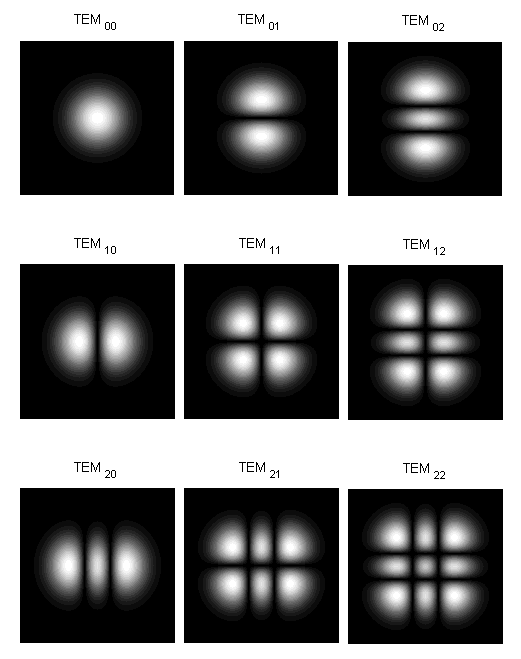
\includegraphics[width=\linewidth]{figures/detectors/TEMmn}
  \caption[Laser modes]{
  \label{f:hermite_gauss}
Basis functions for the cross-sectional distribution of power in a
laser beam.  The lack of symmetry in the higher-order modes can induce
instabilities in the LIGO optics. (\it{Public-domain image taken from
Wikipedia}~\cite{wikipedia:temmn})
}
\end{figure}%

\subsection{Readout}
\label{ssec:readout}

In order to operate correctly the two Fabry-Perot cavities and the
power-recycling mirror must be positioned such that the light is
resonant.  The Michelson must likewise by arranged so that the output
photodetector is on a dark fringe.  When the instrument is in this
state we say it is \emph{locked}, at that point a gravitational wave
will perturb the system within limits and produce light out the
output.  However, the resonances must be very finely tuned and left
untouched the system would quickly fall out of lock due to random
motions of the mirrors.  There is therefore a need for continuous,
active corrections implemented by a system of sensors and servos
throughout the instrument.

Ignoring the OMC there are five degrees of freedom in
figure~\ref{f:ligo}: the two initial test masses, the two end masses,
and the PRC.  Each of these is individually measured and controllable.
However, it is more convenient to consider various linear combinations
of these degrees of freedom:

\begin{itemize}
\item \texttt{DARM}: the differential motion of the two end test masses
\item \texttt{CARM}: the common motion of the two end test masses
\item \texttt{MICH}: the differential motion of the ``small Michelson'' comprising
the ITMs and the beam splitter
\end{itemize}

One of the sensors used to keep the system on resonance is the output
photodector.  Along with this, note that \texttt{DARM} is the quantity
of interest in the experiment, the change in length produced by a
gravitational wave.    It turns outs that rather than reporting the
signal at the photodiode directly a better output is the extent to
which this degree of freedom is off the resonance condition, which is
recorded as \texttt{DARM\_ERR}.  Henceforth, and especially in
chapter~\ref{ch:detchar} we consider this ``the output of the
detector''.  It is not, however, the data stream in which we will
search for gravitational waves.  The detector output needs to be
calibrated with respect to the instrument's frequency response.  This
can be measured by injecting a sinewave of known amplitude into the
system by actuating one of the mirrors, and measuring the amplitude of
\darmerr.  The result is a complicated function of frequency.  This
can then be inverted to map \darmerr back to the true input, the
result is stored as \texttt{LSC\_STRAIN}, and it is that channel on
which gravitational wave searches are performed.

\subsection{Noise sources}

In addition to gravitational wave sources the instrument is subject to
various other influences collectively known as noise.  These sources
are best characterized by their frequency profiles.

\begin{itemize} 

\item \emph{Seismic noise} is due to the coupling of the
instrument to the ground.  Much work has been been done, and much
research continues to be done, to isolate the mirrors from the
environment.  However, the isolation is not complete.  This noise
source dominates at low frequency, rising sharply below 40 Hz in
initial LIGO.  In advanced LIGO we hope to push this so-called
\emph{seismic wall} down to 10 Hz.  This noise source includes the
natural constant vibrations of the Earth, wind blowing over nearby
structures, and anthropogenic sources such as vehicles near the sites,
logging activity, etc.

\item \emph{Thermal noise}. Any system possesses energy proportional to 
the product of Boltzmann's constant and the ambient temperature.  The
energy manifests as random motion of the residual gas in the chambers,
the wires from which the mirrors are hung, and the mirrors themselves.
This produces noise that dominates from 40 Hz to approximately 200 Hz.

\item \emph{Shot noise} is the uncertainty inherent in counting
photons, as discussed above.  It increases with frequency and
dominates above $\approx 1$ kHz.

\end{itemize}

In addition to these broad-band sources of noise there are also
\emph{lines}, particular frequencies at which the noise is much
greater than the three sources above would produce.  Two of the most
significant are

\begin{itemize}
\item \emph{Electrical noise}.  Despite shielding, at 60 Hz there is a
sharp increase in the noise level due to the frequency of the US
electrical grid.
\item \emph{Violin modes}.  Although the wires suspending the mirrors
vibrate over a range of frequencies due to thermal noise, the
suspension system has a resonance at about $340 Hz$, producing much
more noise here.
\end{itemize}

There are also lines at higher harmonics of these frequencies.


\section{Conclusions}

In this chapter we reviewed the basic elements of interferometric
gravitational waves detectors.  In the next chapter we discuss how we
search the data obtained by these detectors for signals of the kind
described in the previous chapter.

